A single writer per location induced a polynomial-time algorithm for the consistency check. Here we show that having two writers per thread makes the problem $\NP$-complete. The $\NP$ upper bound follows by guessing an $\rf$ and $\mo$ and then checking whether the complete execution graph $\ex = \tuple{\E, \po, \rf, \mo}$ satisfies the consistency axioms. When $\rf$ and $\mo$ are already given, this test can be done in polynomial-time~\cite{Tunc2023}. Hence the $\NP$ upper bound follows. The hardness for our $\vm$ problem comes from the fact that we need to \emph{synthesize} suitable $\rf$ and $\mo$ (the analogue in the sequential consistency setting would be the synthesis of an interleaving). For proving hardness, we provide a reduction from 3-CNF-SAT: given a boolean formula $\varphi$ over $k$ variables and $m$ clauses, with each clause being a disjunction of three literals, is there a satisfying assignment for $\varphi$?  We provide two reductions.
\begin{enumerate}
\item Formula $\varphi$ to a partial execution graph $\expartial_\varphi$ with $\mathcal{O}(k)$ threads, and containing at most \emph{three threads} writing to a location (\threewriter). 
\item Formula $\varphi$ to a partial execution graph $\ypartial_\varphi$ with $\mathcal{O}(k + m)$ threads, and containing at most \emph{two threads} writing to a location (\twowriter). 
\end{enumerate}

In both the reductions, we achieve the property that $\varphi$ is satisfiable iff $\expartial_\varphi$ (correspondingly $\ypartial_\varphi$) are $\MemModel$-consistent, for $\MemModel \in \{\sramm, \ramm, \wramm\}$. This shows that the consistency checking problem is $\NP$-complete with a bounded number of writers per location, in fact, even with two writers. The reason we present the first reduction to \threewriter\ is because we get a stronger conditional bound: since the number of threads in $\expartial_\varphi$ is linearly related to the number of variables in $\varphi$, we get a parameterized reduction that helps proving a conditional lower bound under the Exponential Time Hypothesis (ETH). In the reduction to \twowriter\ systems, the number of threads depends both on $k$ (number of variables in the formula) and $m$ (the number of clauses). Hence this reduction cannot be used for the conditional lower bound. 
We will first describe the reduction to three writers and its implications, and then follow up with the second reduction. 

\paragraph*{Notation.} Let the variables used by $\varphi$ be $x_1, \dots, x_k$. The clauses are $C_1, \dots, C_m$. Each clause $C_j$ consists of three literals $(\ell_j^1, \ell_j^2, \ell_j^3)$, where each literal is either a variable $x_i$ or its negation $\neg x_i$. We define $S_{x_i} := \{j \mid C_j \text{ contains } x_i\}$ and $S_{\neg x_i} := \{ j \mid C_j \text{ contains } \neg x_i\}$ as the set of (indices of) clauses containing the literals $x_i$ and $\neg x_i$ respectively.

\section{Fine-grained hardness for  \threewriter\ systems}\label{sec:hardness}
\label{sec:hardness-threewriter}
We consider execution graphs where for each variable $x$ there are at most three threads writing to $x$, that is, at most three threads can have statements of the form $\wt(x, d)$. We will call them \threewriter\ execution graphs. 
Our objective is to show a hardness result stronger than $\NP$-hardness, for the $\vm$ problem under the assumption stated below.

\noindent \textbf{Exponential Time Hypothesis (ETH)}. There is no $2^{o(k)}\cdot (k+m)^{\mathcal{O}(1)}$ algorithm for 3-CNF-SAT, where $k$ is the number of variables, $m$ is the number of clauses~\cite{ImpagliazzoPZ01,Lokshtanov:ETH:2011}.

We prove the following theorem in this section. 

\begin{theorem}\label{thm:eth-hardness}
    Under ETH, there is no $2^{o(k)} \cdot n^{\mathcal{O}(1)}$ algorithm for the $\vm$-problem with $\MemModel \in \{ \sramm, \ramm, \wramm\}$, $k$ being the number of threads, and $n$ the number of events. The result holds even while restricting the input instance to \threewriter\ execution graphs.
\end{theorem}

\paragraph*{Proof strategy.} Given a 3-CNF formula $\varphi$ with $k$ threads and $m$ clauses, we construct a partial execution graph $\expartial_\varphi = \tuple{\E, \po}$ that satisfies the following properties:
\begin{itemize}
\item $\expartial_\varphi$ is \threewriter,
\item the number of threads in $\expartial_\varphi$ is $\mathcal{O}(k)$,
\item the number of events in $\expartial_\varphi$ is $\mathcal{O}(k + m)$, 
\item $\expartial_\varphi \models \MemModel$ iff $\varphi$ is satisfiable, for $\MemModel \in \{\sramm, \ramm, \wramm\}$. 
\end{itemize} 

 
\begin{figure}
\footnotesize%\noindent

\begin{tabular}{c| c}
    $T_i^1$ & $T_i^0$  \\
    $\wt(s_i, 1)$~~&~~$\wt(s_i, 1)$~~ \\
    $\wt(s_i, 2)$~~&~~$\wt(s_i, 2)$~~ \\
    $\wt(v_i, 1)$~~&~~$\wt(v_i, 0)$~~
\end{tabular}
\hfill
\begin{tabular}{c | c }
    $T_{x_i}$~ & ~$T_{\neg x_i}$ \\
        & \\
        $\rd(v_i, 1)$~&~$\rd(v_i, 0)$ \\
        & \\
        $\wt(c_j, 1)$ ~&~ $\wt(c_j, 1)$ \\
        $\forall j \in S_{x_i}$ ~&~  $\forall j \in S_{\neg x_i}$ 
\end{tabular}
\hfill
\begin{tabular}{c}
    $T_f$ \\
    $\rd(c_1, 1)$ \\
    $\cdots$ \\
    $\rd(c_m, 1)$ \\
    $\rd(s_1, 2)$ \\
    $\rd(s_1, 1)$ \\
    $\cdots$ \\
    $\rd(s_k, 2)$ \\
    $\rd(s_k, 1)$ 
\end{tabular}
 \caption{Threads in the reduction, for $i \in \{1, 2, \dots, k\}$ }
   \label{tab:reduction-threads-ra}
\end{figure}

Thus, if there was a $2^{o(k)} \cdot n^{\mathcal{O}(1)}$ algorithm for the $\vm$ problem, we could solve 3-CNF-SAT in $2^{o(k)}.(k+m)^{\mathcal{O}(1)}$ time: from $\varphi$, construct the $\vm$ instance in $\mathcal{O}(k + m)$ time, and then use the $2^{o(k)} \cdot (k+m)^{\mathcal{O}(1)}$ procedure for $\vm$, thereby contradicting ETH. To show the last item above, we make use of what is known in the literature as a \emph{range reduction}~\cite{ChakrabortyKMP24}: using Lemma~\ref{lem:sra-ra-wra-relationship}, it is enough to show that if $\varphi$ has a satisfying assignment, then $\expartial \models \sramm$, and if $\varphi$ does not have a satisfying assignment, then $\expartial \not \models \wramm$. 

\paragraph*{The reduction.} 
 For every variable $x_i$, we introduce four threads $T_i^1$, $T_i^0$, $T_{x_i}$ and $T_{\neg x_i}$, as shown in Figure~\ref{tab:reduction-threads-ra}. Apart from these, there is a special thread $T_f$. 

The statements $\wt(v_i, 1)$ and $\wt(v_i,0)$ in $T_i^1$ and $T_i^0$ encode variable $x_i$ being set to \emph{true} and \emph{false} respectively. Thread $T_{x_i}$ has a read statement $\rd(v_i,1)$ (reading \emph{true} for $x_i$) and sets all clauses containing $x_i$ to true, using the statement $\wt(c_j, 1)$ for all $j \in S_{x_i}$. Similarly, thread $T_{\neg x_i}$ reads $\rd(v_i, 0)$ (\emph{false} for $x_i$) and sets all clauses containing $\neg x_i$ to true. Finally the thread $T_{f}$ needs to make sure that all clauses are set to true, hence the read statements $\rd(c_1, 1), \dots, \rd(c_m, 1)$.  The main challenge is to encode a valid assignment, where every variable is assigned a unique truth value: to do this, we need to ensure that there are no two distinct reads $\rd(c_{j}, 1)$ and $\rd(c_\ell, 1)$ in $T_f$ which read from some $T_{x_i}$ and its negation $T_{\neg x_i}$.
This is where the rest of the statements, using $s_i$ become useful, as we elaborate in the proofs below.

\begin{lemma}\label{lem:wra-eth}
If  $\expartial_\varphi \models \wramm$, then $\varphi$ has a satisfying assignment. 
\end{lemma}
\begin{proof} 
    If $\expartial_\varphi \models \wramm$ there is an $\rf$ function which satisfies porf-acyclicity and weak-read-coherence. We need to prove that this $\rf$ encodes a valid satisfying assignment. This can be shown by proving that there are no two distinct reads $\rd(c_j, 1)$ and $\rd(c_\ell, 1)$ which read from $T_{x_i}$ and $T_{\neg x_i}$ for some variable $x_i$, since it gives the following assignment: $A(x_i) = true$ if some read event $\rd(c_j, 1)$ reads from the write in $T_{x_i}$; $A(x_i) = false$ otherwise. Moreover, the assignment $A$ is satisfying since every clause is made  true by this assignment.
    

    Let us now prove the property. Suppose $\rd(c_j, 1)$ and $\rd(c_\ell, 1)$ read from $T_{x_i}$ and $T_{\neg x_i}$ respectively. Since $\rd(c_j, 1)$ reads from $T_{x_i}$, there is an $\hb$ path from $T_i^1$ to $\rd(c_j, 1)$ due to the $\rf$ edges: $\wt(v_i, 1) \xra{\rf} \rd(v_i, 1)$ and $T_{x_i}: \wt(c_j, 1) \xra{\rf} \rd(c_j, 1)$. Similarly, there is an $\hb$ path from $T_i^0$ to $\rd(c_\ell, 1)$. Hence there is an $\hb$ path from both $T_i^1$ and $T_i^0$ to the event $\rd(s_i, 1)$ in $T_f$. Since the only matching write $\wt(s_i, 1)$ appears above $\wt(s_i, 2)$ in these threads, any assignment to $\rd(s_i, 1)$ violates weak-read-coherence, a contradiction to the hypothesis that $\rf$ satisfies weak-read-coherence.
\end{proof}

\begin{restatable}{lemma}{lemsatimpliessra}
    \label{lem:sat-implies-sra}
If $\varphi$ has a satisfying assignment, then $\expartial_\varphi \models \sramm$. 
\end{restatable}
\begin{proof}
Suppose $\varphi$ has a satisfying assignment $A$. We need to synthesize $\rf$ and $\mo$ such that the resulting execution graph satisfes porf-acyclicity, strong-write-coherence and read-coherence. Since $A$ is a satisfying assignment, for every clause $C_j$ there is a literal $\ell_j$ that is made true. Let $\rf^{-1}(\rd(c_j, 1))$ be the write event $\wt(c_j, 1)$ in $T_{\ell_j}$. Assigning writes this way introduces an $\hb$ path from $T_i^{A(x_i)}$ to $T_f$ for all variables that are indeed being utilized to make the clauses true. Importantly, there is no $\hb$ path created from $T_{i}^{\neg A(x_i)}$ to the thread $T_f$. Therefore, the read event $\rd(s_i, 2)$ can read from the write in $T_i^{A(x_i)}$ and $\rd(s_i, 1)$ can read from the unused thread $T_i^{\neg A(x_i)}$. This gives an $\rf$ which satisfies weak-read-coherence. By design of the execution graph, the $\rf$ also satisfies porf-acyclicity. For the lemma, we require to prove strong-write-coherence and read-coherence. For this we need to also synthesize an $\mo$. 
Consider any  $\mo$ relation that respects the following orders:
    \begin{itemize}[leftmargin=0.1em]
    \item $T_{i}^{A(x_i)}: \wt(s_i, 1) \xra{\mo} T_i^{\neg A(x_i)}: \wt(s_i, 1) \xra{\mo}T_{i}^{\neg A(x_i)}: \wt(s_i, 2);  T_i^{A(x_i)}: \wt(s_i, 2) \xra{\mo} T_i^{\neg A(x_i)}: \wt(s_i, 1)$,
    \item For each clause $j$ there are three threads writing $\wt(c_j, 1)$.  For each clause $C_j$ choose a specific literal $\ell_j$ that is made true by the satisfying assignment $A$. The $\mo$ relation orders the other write statements $\wt(c_j, 1)$ before $T_{\ell_j}: \wt(c_j, 1)$. 
    \end{itemize} 
A concrete example of the synthesis is presented below. It shows a complete execution graph along with the synthesis of $\rf$ and $\mo$ edges.
\paragraph*{Illustration}\label{app:hardness-example}
\begin{table}[h]
    
\noindent
\begin{minipage}{0.15\textwidth}
\centering
\begin{tabular}{c | c}
    $T_1^1$ & $T_1^0$ \\
    $\wt(s_1,1)$~& ~$\wt(s_1,1)$ \\ 
    $\wt(s_1,2)$~& ~$\wt(s_1,2)$ \\ 
    $\wt(v_1, 1)$~& ~$\wt(v_1, 0)$ \\

\end{tabular}
\vspace{.1cm}

\begin{tabular}{c | c}
    $T_2^1$ & $T_2^0$ \\
    $\wt(s_2,1)$~& ~$\wt(s_2,1)$ \\ 
    $\wt(s_2,2)$~& ~$\wt(s_2,2)$ \\ 
    $\wt(v_2, 1)$~& ~$\wt(v_2, 0)$ \\
\end{tabular}
\vspace{.1cm}

\begin{tabular}{c | c}
    $T_3^1$ & $T_3^0$ \\
    $\wt(s_3,1)$~& ~$\wt(s_3,1)$ \\ 
    $\wt(s_3,2)$~& ~$\wt(s_3,2)$ \\ 
    $\wt(v_3, 1)$~& ~$\wt(v_3, 0)$ \\
   
\end{tabular}

\end{minipage}
\hfill
\begin{minipage}{0.15\textwidth}
\centering
\centering
\begin{tabular}{c | c}
    $T_{x_1}$ & $T_{\neg x_1}$ \\
    $\rd(v_1,1)$ ~& ~$\rd(v_1,0)$ \\ 
    $\wt(c_1,1)$~ &  \\ 
    $\wt(c_2, 1)$~&  \\

\end{tabular}
\vspace{.1cm}

\begin{tabular}{c | c}
   $T_{x_2}$ & $T_{\neg x_2}$ \\
    $\rd(v_2,1)$ ~& ~$\rd(v_2,0)$ \\ 
    $\wt(c_1,1)$~ & ~$\wt(c_2,1)$ \\ 
    
\end{tabular}
\vspace{.1cm}

\begin{tabular}{c | c}
    $T_{x_3}$ & $T_{\neg x_3}$ \\
    $\rd(v_3,1)$ ~& ~$\rd(v_3,0)$ \\ 
    $\wt(c_1,1)$~ & ~$\wt(c_2,1)$ \\ 
    
   
\end{tabular}
\end{minipage}
\hfill
\begin{minipage}{0.15\textwidth}
\centering
\begin{tabular}{c}
    $T_f$ \\
    $\rd(c_1, 1)$ \\
    $\rd(c_2, 1)$ \\
    $\rd(s_1, 2)$ \\
    $\rd(s_1, 1)$ \\
    $\rd(s_2, 2)$ \\
    $\rd(s_2, 1)$ \\
    $\rd(s_3, 2)$ \\
    $\rd(s_3, 1)$ \\

\end{tabular}
\end{minipage}
\vspace{2em}
\caption{$\varphi=(x_1\lor x_2\lor x_3)\land (x_1 \lor \neg x_2\lor \neg x_3)$}
    \label{tab:example-finegrainedwra}
\end{table}

Table~\ref{tab:example-finegrainedwra} gives an instance of the construction of $\expartial$ for the fine-grained hardness reduction for \threewriter~ and (Figure~\ref{example-Execution-ra}) gives the complete execution graph for it. The execution graph is constructed for $x_1=1, x_2=0, x_3=0$, a satisfying assignment for $\varphi$. The $\rf$ and $\mo$-edges follow the rule of construction for them given in the reduction we discussed before. The $\rf$ synthesis is as follows:
\begin{itemize}
    \item $\tuple{T_{x_1}:\wt(c_1,1)}~\rf~\tuple{T_f:\rd(c_1,1)}$, $\tuple{T_{x_1}:\wt(c_2,1)}~\rf~\tuple{T_f:\rd(c_2,1)}$
    \item $\tuple{T_1^1:\wt(s_1,2)}~\rf~\tuple{T_f:\rd(s_1,2)}$, $\tuple{T_1^0:\wt(s_1,1)}~\rf~\tuple{T_f:\rd(s_1,1)}$
    \item $\tuple{T_2^0:\wt(s_2,2)}~\rf~\tuple{T_f:\rd(s_2,2)}$, $\tuple{T_2^1:\wt(s_2,1)}~\rf~\tuple{T_f:\rd(s_2,1)}$
    \item $\tuple{T_3^0:\wt(s_3,2)}~\rf~\tuple{T_f:\rd(s_3,2)}$, $\tuple{T_3^1:\wt(s_3,1)}~\rf~\tuple{T_f:\rd(s_3,1)}$
\end{itemize}

All other $\rf$-edges are trivial. They are not reflected in Figure~\ref{example-Execution-ra}. Let us construct the $\mo$-edges.
\begin{itemize}
 \item $\tuple{T_1^1:\wt{s_1,2}} \xra{\mo}\allowbreak \tuple{T_1^0:\wt{s_1,1}}$ , $\tuple{T_1^1:\wt{s_1,1}} \xra{\mo}\allowbreak \tuple{T_1^0:\wt{s_1,1}}$
 
 \item $\tuple{T_j^0:\wt{s_j,2}} \xra{\mo}\allowbreak \tuple{T_j^1:\wt{s_j,1}}$, $\tuple{T_j^0:\wt{s_j,1}} \xra{\mo}\allowbreak \tuple{T_j^1:\wt{s_j,1}}$ for $j=2,3$
 
 \item $\tuple{T_{x_j}:\wt{c_1,1}} \xra{\mo}\allowbreak \tuple{T_{x_1}:\wt{c_1,1}}$, $\tuple{T_{x_j}:\wt{c_2,1}} \xra{\mo}\allowbreak \tuple{T_{x_1}:\wt{c_2,1}}$ for $j=1,2$.
\end{itemize}

Other $\mo$ edges follow the direction of $\po$ and are not explicitly constructed in Figure~\ref{example-Execution-ra}. %Note that the resulting execution graph satisfies all the memory axioms of $\sramm$ (Refer Table~\ref{table:ax:models-2}).


\begin{figure*}% 
\begin{center}
 \begin{tikzpicture}[scale =1,yscale=2, 
    op/.style={draw, fill=white, rounded corners, minimum width=1.25cm, minimum height=0.55cm, 
               inner sep=2pt, font=\small},
    thread/.style={font=\small\bfseries},
    >=stealth
]

% ------------------------------------------------------------
% First group: T_i^1 and T_i^0
% ------------------------------------------------------------

% T_1^1 / T_1^0
\node[thread] (T11) at (0, 0.9) {$T_1^1$};
\node[thread] (T10) at (2.0, 0.9) {$T_1^0$};

\node[op] (s11a) at (0, 0.2) {$\wt(s_1,1)$};
\node[op] (s11b) at (0,-0.5) {$\wt(s_1,2)$};
\node[op] (v11)  at (0,-1.2) {$\wt(v_1,1)$};

\draw[po] (s11a) to (s11b);
\draw[po] (s11b) to (v11);



\node[op] (s10a) at (2.0, 0.2) {$\wt(s_1,1)$};
\node[op] (s10b) at (2.0,-0.5) {$\wt(s_1,2)$};
\node[op] (v10)  at (2.0,-1.2) {$\wt(v_1,0)$};

\draw[po] (s10a) to (s10b);
\draw[po] (s10b) to (v10);

\draw[mo] (s11b) to node[above] {$\mo$} (s10a);
\draw[mo] (s11a) to (s10a);

% T_2^1 / T_2^0
\node[thread] (T21) at (0,-2.4) {$T_2^1$};
\node[thread] (T20) at (2.0,-2.4) {$T_2^0$};

\node[op] (s21a) at (0,-3.1) {$\wt(s_2,1)$};
\node[op] (s21b) at (0,-3.8) {$\wt(s_2,2)$};
\node[op] (v21)  at (0,-4.5) {$\wt(v_2,1)$};

\draw[po] (s21a) to (s21b);
\draw[po] (s21b) to (v21);

\node[op] (s20a) at (2.0,-3.1) {$\wt(s_2,1)$};
\node[op] (s20b) at (2.0,-3.8) {$\wt(s_2,2)$};
\node[op] (v20)  at (2.0,-4.5) {$\wt(v_2,0)$};

\draw[po] (s20a) to (s20b);
\draw[po] (s20b) to (v20);
\draw[mo] (s20b) to node[above] {$\mo$} (s21a);
\draw[mo] (s20a) to (s21a);

% T_3^1 / T_3^0
\node[thread] (T31) at (0,-5.7) {$T_3^1$};
\node[thread] (T30) at (2.0,-5.7) {$T_3^0$};

\node[op] (s31a) at (0,-6.4) {$\wt(s_3,1)$};
\node[op] (s31b) at (0,-7.1) {$\wt(s_3,2)$};
\node[op] (v31)  at (0,-7.8) {$\wt(v_3,1)$};

\draw[po] (s31a) to (s31b);
\draw[po] (s31b) to (v31);

\node[op] (s30a) at (2.0,-6.4) {$\wt(s_3,1)$};
\node[op] (s30b) at (2.0,-7.1) {$\wt(s_3,2)$};
\node[op] (v30)  at (2.0,-7.8) {$\wt(v_3,0)$};

\draw[po] (s30a) to (s30b);
\draw[po] (s30b) to (v30);
\draw[mo] (s30b) to node[above] {$\mo$} (s31a);
\draw[mo] (s30a) to (s31a);
% ------------------------------------------------------------
% Second group: T_xi and T_not xi
% ------------------------------------------------------------

% T_x1 / T_not x1
\node[thread] (Tx1)  at (5.0, 0.9) {$T_{x_1}$};
\node[thread] (Tnx1) at (7.0, 0.9) {$T_{\neg x_1}$};

\node[op] (rv11) at (5.0,0.2) {$\rd(v_1,1)$};
\node[op] (c11)  at (5.0,-0.5) {$\wt(c_1,1)$};
\node[op] (c21)  at (5.0,-1.2) {$\wt(c_2,1)$};

\draw[po] (rv11) to (c11);
\draw[po] (c11) to (c21);

\node[op] (rv10) at (7.0,0.2) {$\rd(v_1,0)$};

% T_x2 / T_not x2
\node[thread] (Tx2)  at (5.0,-2.4) {$T_{x_2}$};
\node[thread] (Tnx2) at (7.0,-2.4) {$T_{\neg x_2}$};

\node[op] (rv21) at (5.0,-3.1) {$\rd(v_2,1)$};
\node[op] (c12)  at (5.0,-3.8) {$\wt(c_1,1)$};

\draw[po] (rv21) to (c12);


\node[op] (rv20) at (7.0,-3.1) {$\rd(v_2,0)$};
\node[op] (c22)  at (7.0,-3.8) {$\wt(c_2,1)$};

\draw[po] (rv20) to (c22);

% T_x3 / T_not x3
\node[thread] (Tx3)  at (5.0,-5.7) {$T_{x_3}$};
\node[thread] (Tnx3) at (7.0,-5.7) {$T_{\neg x_3}$};

\node[op] (rv31) at (5.0,-6.4) {$\rd(v_3,1)$};
\node[op] (c13)  at (5.0,-7.1) {$\wt(c_1,1)$};

\draw[po] (rv31) to (c13);

\node[op] (rv30) at (7.0,-6.4) {$\rd(v_3,0)$};
\node[op] (c23)  at (7.0,-7.1) {$\wt(c_2,1)$};

\draw[po] (rv30) to (c23);
\draw[mo, bend left=45] (c12.west) to (c11);
\draw[mo, bend left=5] (c22.west) to (c21);
\draw[mo, bend left=50] (c13.west) to (c11.west);
\draw[mo, bend right=55] (c23.east) to (c21.east);

% ------------------------------------------------------------
% Final thread T_f
% ------------------------------------------------------------

\node[thread] (Tf) at (10.0,0.9) {$T_f$};

\node[op] (fc1) at (10.0,0.2) {$\rd(c_1,1)$};
\node[op] (fc2) at (10.0,-0.5) {$\rd(c_2,1)$};
\node[op] (fs12) at (10.0,-1.2) {$\rd(s_1,2)$};
\node[op] (fs11) at (10.0,-1.9) {$\rd(s_1,1)$};
\node[op] (fs22) at (10.0,-2.6) {$\rd(s_2,2)$};
\node[op] (fs21) at (10.0,-3.3) {$\rd(s_2,1)$};
\node[op] (fs32) at (10.0,-4.0) {$\rd(s_3,2)$};
\node[op] (fs31) at (10.0,-4.7) {$\rd(s_3,1)$};

%po for Tf
\draw[po] (fc1) to (fc2);
\draw[po] (fc2) to (fs12);
\draw[po] (fs12) to (fs11);
\draw[po] (fs11) to (fs22);
\draw[po] (fs22) to (fs21);
\draw[po] (fs21) to (fs32);
\draw[po] (fs32) to (fs31);

%rf edges

\draw[rf] (c11) to (fc1);
\draw[rf] (c21) to (fc2);
\draw[rf, bend right=8] (s11b) to (fs12);
\draw[rf, bend right=25] (s10a) to (fs11);
\draw[rf, bend left=10] (s20b) to (fs22);
\draw[rf, bend left=10] (s21a) to (fs21);
\draw[rf, bend left=0] (s30b) to (fs32);
\draw[rf, bend left=0] (s31a) to (fs31);
\end{tikzpicture}%
\end{center}
\caption{Execution graph for Table~\ref{tab:example-finegrainedwra}:The trivial $\rf$-edges are omitted}
\label{example-Execution-ra}
\end{figure*}%
 


It can be shown that the constructed $\rf$ and $\mo$ satisfy strong-write-coherence and read-coherence.

\paragraph*{Strong-write-coherence.} We will show that the constructed $\rf$ and $\mo$ satisfy strong-write-coherence, that is acyclicity of $\hb \cup
 \mo$. Suppose not. There is a cycle $\mathcal{C}$ consisting of $\po$, $\rf$ and $\mo$ edges (thereby violating strong-write-coherence). Since we have seen that there is no $\po \cup \rf$ cycle, cycle $\mathcal{C}$ should contain an $\mo$ edge.  An edge  $\tuple{T_{i}^{A(x_i)}: \wt(s_i, 1)} ~\mo~\tuple{T_i^{\neg{A(x_i)}}: \wt(s_i, 1)}$ cannot be present in $\mathcal{C}$ since there can be no incoming $\po$ or $\rf$ edge to $\tuple{T_{i}^{A(x_i)}: \wt(s_i, 1)}$. Now, consider an edge $\tuple{T_{i}^{A(x_i)}: \wt(s_i, 2)}~\mo~\allowbreak \tuple{T_{i}^{\neg{A(x_i)}}: \wt(s_i, 1)}$. 
  The only incoming edge to $\tuple{T_{i}^{A(x_i)}: \wt(s_i, 2)}$ is a $\po$ edge from $\tuple{T_{i}^{A(x_i)}: \wt(s_i, 1)}$, and there can be no $\po$ or $\rf$ edges into the latter event. Hence, even the second type of $\mo$ edges cannot be present in $\mathcal{C}$. 
This leaves us with $\mo$ edges of the form $\tuple{T_{\ell'}: \wt(c_j, 1)} ~\mo~\allowbreak  \tuple{T_{\ell_j}: \wt(c_j,1)}$. Notice that from the latter event, $\tuple{T_{\ell_j}: \wt(c_j, 1)}$ the only outgoing edges are to $T_f$, and from $T_f$, there are no outgoing edges, hence there is no path from an event in $T_f$ to $\tuple{T_{\ell'}: \wt(c_j, 1)}$. This proves that such an $\mo$ edge cannot be part of an $\hb \cup \po$ cycle too. We conclude that there are no $\hb \cup \mo$ cycles. 


    \paragraph*{Read-coherence.} Finally, we need to prove read-coherence, i.e., $\irr(\rf^{-1}; \mo_x; \hb)$. If read coherence is violated, there is a read event $r$, and two write events $w, w'$ such that $w~\rf~r$, $w~\mo~w'$ and $w'~\hb~r$. Such a violation can potentially happen on variables which have multiple write events: in our case $s_i$ and $c_j$.
    
    To do this, let us check what each reads on $s_i$ and $c_j$ observes. Note that no read observes a value that is $\mo$-overwritten in its happens-before past. 
    \begin{itemize}[leftmargin=0.1em]
    \item By construction $\tuple{T_f: \rd(s_i, 2)}$ can observe $\tuple{T_i^{A(x_i)}:\wt(s_i,2)}$ but not $\tuple{T_i^{\neg A(x_i)}:\wt(s_i,1)}$. Therefore there is no write event $\mo$-later than $\tuple{T_i^{A(x_i)}: \wt(s_i, 2)}$ that is observed by $\tuple{T_f: \rd(s_i, 2)}$. 
    \item For the read event $\tuple{T_f: \rd(s_i, 1)}$, all writes to $s_i$ except $\tuple{T_i^{\neg{A(x_i)}}: \wt(s_i, 2)}$ are visible to it. Moreover, the event $\tuple{T_i^{\neg A(x_i)}: \wt(s_i, 1)}$ that writes to it is the $\mo$-latest in the view.
    \item For the variable $c_j$, $\tuple{T_f: \rd(c_j, 1)}$ observes only the write $\tuple{T_{\ell_j}: \wt(c_j, 1)}$ when some literal literal $\ell_j$ satisfies $C_j$ under $A$. All other writes to $c_j$ occur $\mo$ before this write.
    \end{itemize}
    
    This shows that the constructed $\rf$ and $\mo$ are consistent with $\sramm$.
\end{proof}

We can modify the  construction of $\expartial_{\varphi}$ for $\threewriter$ to build an execuion graph for $\varphi$ which would have only two threads writing to each variable. This will be the task  behind the reduction to $\twowriter$ systems as we will see in the next section. 

 %%%%%%%%%NP-hardness%%%%%%%%%%
\subsection{Hardness for  \twowriter\ systems}
\label{sec:hardness-twowriter}

The reduction in Section~\ref{sec:hardness-threewriter} involved \threewriter\ systems.
Mainly, each clause variable $c_j$ was written by three threads corresponding to its three literals. Here, our objective is to prove hardness even when there are atmost two threads writing to each variable. We will now reduce 3-CNF-SAT to the consistency testing problem for \twowriter~ systems. However, in this reduction, a formula $\varphi$ with $k$ threads and $m$ clauses yields an execution graph with $\mathcal{O}(k + m)$ theads. While this still proves $\NP$-hardness, it does not give the stronger hardness under ETH, parameterized by the number of threads. 

\begin{theorem}
\label{thm:two-writer-hardness}
    The $\vm$ problem is $\NP$-complete for $\MemModel \in \{\sramm, \ramm, \wramm\}$, even when restricted to \twowriter\ execution graphs.
\end{theorem}



The key challenge in proving the hardness is to reduce the number of threads writing to each clause variable $c_j$ from three (one for each literal in the clause) to at most two, while still encoding the satisfiability of the 3-CNF formula. This can be achieved by introducing one auxiliary variable $d_j$ per clause. Suppose $C_j = (\ell_j^1 \vee \ell_j^2 \vee \ell_j^3)$. In all the reductions of Section~\ref{sec:hardness-threewriter}, there are three threads $T_{\ell_j^1}, T_{\ell_j^2}$ and $T_{\ell_j^3}$. We make the following changes to constructions of $\expartial_\varphi$ in Section~\ref{sec:hardness-threewriter}.

\begin{itemize}[leftmargin=0.1em]
\item Replace $\wt(c_j, 1)$ in $T_{\ell_j^3}$ with $\wt(d_j, 1)$, i.e., in the third literal, the write is on $d_j$.
\item Add a new thread $T_{j}$ with two events as follows: $\rd(c_j, 1)~;~\wt(d_j, 1)$
\item Finally, in $T_f$, replace all $\rd(c_j, 1)$ with $\rd(d_j, 1)$
\end{itemize}
Figure~\ref{fig:two-writer} reflects the changes and the full thread construction for the reduction to $\twowriter$.

\begin{figure}[t]
\centering
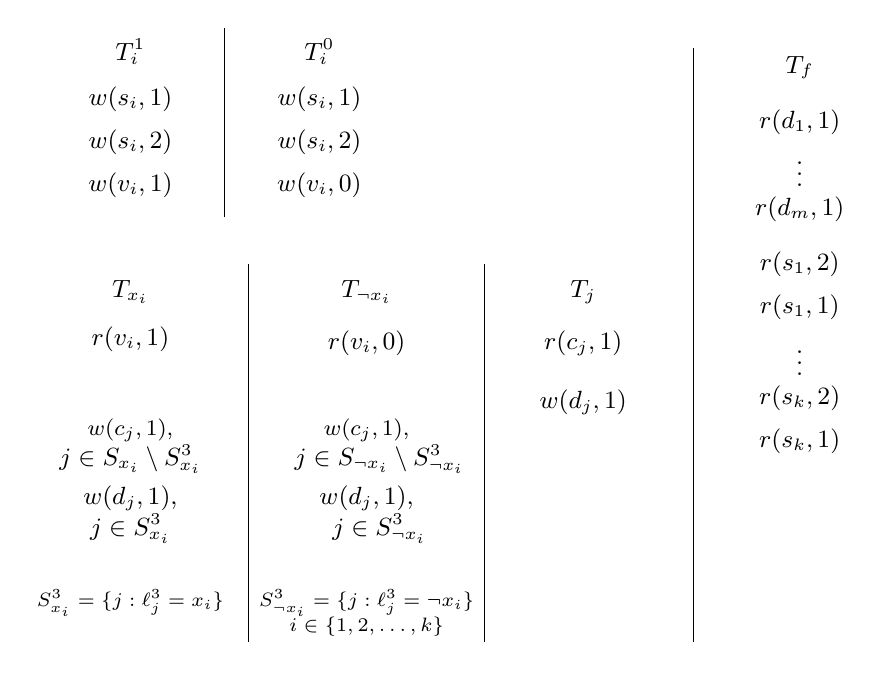
\begin{tikzpicture}[
    every node/.style={font=\small}
]

% =========================================================
% T_i^{1}
% =========================================================

\node at (0,0) {$T_i^1$};

\node at (0,-0.60) {$w(s_i,1)$};
\node at (0,-1.15) {$w(s_i,2)$};
\node at (0,-1.70) {$w(v_i,1)$};


% =========================================================
% T_i^{0}
% =========================================================

\node at (2.4,0) {$T_i^0$};

\node at (2.4,-0.60) {$w(s_i,1)$};
\node at (2.4,-1.15) {$w(s_i,2)$};
\node at (2.4,-1.70) {$w(v_i,0)$};


% vertical separator
\draw (1.2,0.30) -- (1.2,-2.10);


% =========================================================
% T_{x_i}
% =========================================================

\node at (0,-3.05) {$T_{x_i}$};

\node at (0,-3.65) {$r(v_i,1)$};

\node[align=center] at (0,-5.45)
{
\footnotesize $w(c_j,1)$,\\ $j\in S_{x_i}\setminus S_{x_i}^{3}$\\[3pt]
$w(d_j,1)$,\\
$j\in S_{x_i}^{3}$
};



\node[align=center] at (0,-7)
{\scriptsize $S_{x_i}^{3}=\{j:\ell_j^3=x_i\}$};


% =========================================================
% T_{\neg x_i}
% =========================================================

\node at (3.0,-3.05) {$T_{\neg x_i}$};

\node at (3.0,-3.70) {$r(v_i,0)$};

\node[align=center] at (3.0,-5.45)
{
\footnotesize $w(c_j,1)$,\\ \quad $j\in S_{\neg x_i}\setminus S_{\neg x_i}^{3}$\\[3pt]
$w(d_j,1)$,\\ \quad $j\in S_{\neg x_i}^{3}$
};

\node[align=center] at (3.0,-7)
{\scriptsize $S_{\neg x_i}^{3}=\{j:\ell_j^3=\neg x_i\}$};



% vertical separator
\draw (1.50,-2.70) -- (1.50,-7.5);


% =========================================================
% T_j
% =========================================================

\node at (5.75,-3.05) {$T_j$};

\node at (5.75,-3.70) {$r(c_j,1)$};
\node at (5.75,-4.45) {$w(d_j,1)$};


% vertical separator
\draw (4.50,-2.70) -- (4.50,-7.5);


% =========================================================
% T_f
% =========================================================

\node at (8.5,-0.20) {$T_f$};

\node at (8.5,-0.90) {$r(d_1,1)$};
\node at (8.5,-1.45) {$\vdots$};
\node at (8.5,-2.00) {$r(d_m,1)$};

\node at (8.5,-2.70) {$r(s_1,2)$};
\node at (8.5,-3.25) {$r(s_1,1)$};

\node at (8.5,-3.85) {$\vdots$};

\node at (8.5,-4.40) {$r(s_k,2)$};
\node at (8.5,-4.95) {$r(s_k,1)$};


% vertical separator
\draw (7.15,0.05) -- (7.15,-7.5);


% =========================================================
% Index
% =========================================================

\node at (3,-7.3)
{\scriptsize $i\in\{1,2,\ldots,k\}$};


\end{tikzpicture}

\caption{Threads in the 2-Writer reduction, for
$i\in\{1,2,\ldots,k\}$.}
\label{fig:two-writer}
\end{figure}


Notice that due to the introduction of the new threads $T_j$, the total number of threads also depends on the number of clauses $m$. Let the resulting partial execution graph be called $\ypartial_\varphi$. Then we want to show that $\varphi$ has a satisfying assignment iff $\ypartial_\varphi$ has a complete execution that satisfies the axioms of $\sramm$, $\ramm$ and $\wramm$. We again use range reduction to prove the following two lemmas.

\begin{lemma}
If  $\ypartial_\varphi \models \wramm$, then $\varphi$ has a satisfying assignment. 
\end{lemma}
\begin{proof}
The proof proceeds similar to Lemma~\ref{lem:wra-eth}. We need to argue that if there is an $\rf$ that satisfies weak-read-coherence, then there cannot be two distinct reads $\rd(d_{j}, 1)$ and $\rd(d_{p}, 1)$ in $T_f$ that (directly or indirectly) read from threads corresponding to both a literal and its negation for some variable $x_i$. The $\rd(d_j, 1)$ event in $T_f$ can either read from  $T_{\ell_j^3}$ or from $T_{j}$. Similarly, $\rd(d_p, 1)$ can read from $T_{\ell_p^3}$ or $T_p$. If it so happens that the two threads from which $\rd(d_{j}, 1)$ and $\rd(d_{p}, 1)$ read from are of the form $T_{x_i}$ and $T_{\neg x_i}$, then both $\tuple{T_i^0: \wt(s_i, 2)}$ and $\tuple{T_i^1: \wt(s_i, 2)}$ are in the view of $\tuple{T_f: \rd(s_i, 2)}$. Then, since the execution satisfies weak-read-coherence, there is no write event available for $\tuple{T_f: \rd(s_i, 1)}$. A contradiction. Hence the set of literals making the clauses true in $T_f$ encode a satisfying assignment. 
\end{proof}

\begin{lemma}
If $\varphi$ has a satisfying assignment, then $\ypartial_\varphi^{\ramm} \models \sramm$. 
\end{lemma}
\begin{proof}
Let $A$ be a satisfying assignment. The $\rf$ and $\mo$ relations on events with variables $s_i$ remains the same as in the proof of Lemma~\ref{lem:sat-implies-sra}. There are changes for $c_j$ and $d_j$. Consider a clause $C_j$.
\begin{itemize}
\item If $A$ makes $\ell_j^3$ true then:
\begin{itemize}
\item $\tuple{T_{\ell_j^3}: \wt(d_j, 1)}~\rf~\tuple{T_f: \rd(d_j, 1)}$,
\item Choose an arbitrary $\wt(c_j, 1)$ for $\tuple{T_j: \rd(c_j, 1)}$
\end{itemize}
\item Else, $A$ makes one of the first two literals of $C_j$ true. Arbitrarily pick one $\ell_j^i$, for $i \in \{1,2\}$:  
\begin{itemize}
\item $\tuple{T_{\ell_j^i}: \wt(c_j, 1)}~\rf~ \tuple{T_j: \rd(c_j, 1)}$,
\item $\tuple{T_{j}:\wt(d_j, 1)}~\rf~\tuple{T_f: \rd(d_j, 1)}$
\end{itemize}
\end{itemize}
For every variable-value pair, there are atmost two writes. With the $\rf$ picked as above, the $\mo$ relation gets fixed: the unused write is $\mo$-before the used write.

Clearly, the $\rf$ relation agrees with $\po$ and hence does not violate porf-acyclicity. We need to prove strong-write-coherence and read-coherence as in the proof of Lemma~\ref{lem:sat-implies-sra}.

\paragraph*{Strong-write-coherence.} 
Suppose, for contradiction, that there is a cycle in $\hb \cup \mo$. As in Lemma~\ref{lem:sat-implies-sra}, the only possible $\mo$ edges are between the two writes to $s_i$, $c_j$, or $d_j$. For $s_i$, the argument is identical to the $\threewriter$ case: the only incoming edges to the earlier write are from $\po$, and there are no cycles. For $c_j$ and $d_j$, each has at most two writers, and the $\mo$-later event leads to $T_f$ from which there is no path back to the $\mo$-earlier event. Thus, no cycle can be formed. Therefore, strong-write-coherence holds.

\paragraph*{Read-coherence.}
Suppose, for contradiction, that there is a violation of read-coherence: there exists a read $r$ and two writes $w, w'$ to the same variable such that $w~\rf~r$, $w~\mo~w'$, and $w'~\hb~r$. As before, this can only occur for variables $s_i$, $c_j$, or $d_j$. For $s_i$, the argument is unchanged from Lemma~\ref{lem:sat-implies-sra}. For $c_j$ and $d_j$, the view of each read contains only the $\rf$-used write, and the other write (if any) is $\mo$-before and not visible to the read. Thus, no such violation can occur.

The above two lemmas show that the constructed $\rf$ and $\mo$ are consistent with $\sramm$. 
\end{proof}

\smallskip
\section{Discussion}\label{ra-discuss}

We have presented a trichotomy of the landscape, with $\onewriter$ solved in polynomial-time, $\twowriter$ being NP-complete, and $\threewriter$ having a stronger lower bound under the Exponential-Time-Hypothesis (ETH). Our presentation works for $\ramm$ and its close variants $\sramm$ and $\wramm$.

A milder variant of the problem studies the complexity when the reads-from relation $\rf$ is also given. Then the question is to synthesize an mo such that the axioms can be satisfied. This “$\rf$-given” problem can be solved in polynomial time \cite{Tunc2023}, under no restrictions on the execution graphs. When rf is not provided
apriori, while the general problem is known to be NP-hard \cite{gibbons}, no subclass or
bounded variant with a polynomial-time algorithm is known in the literature (to
the best of my knowledge). We have shown that the $\onewriter$ subclass lends itself to a polynomial-time algorithm. In the next chapter we shall look at the $\rlxmm$ version of the $\vm$ problem and obtain similar trichotomy of results. 
